\section{Jagoda Flejmer}
\label{sec:jagoda_flejmer}
%\begin{document}

\subsection{Zdjęcia}
Zdjęcia są, różne rozmiary mogą mieć: (patrz \ref{fig:noga} oraz \ref{fig:pain} ), niestety przez tak duży rozmiar obrazka \ref{fig:pain} LaTeX za najlepsze miejsce, uniknięcię pustej przestrzeni, uznaje następną stronę\\
                \begin{figure}[htbp] %htbp - obraz dokładnie w tym miejscu (priorytetyzacja wyboru przez użytkownika z kolejnością liter: h - w tym miejscu, t - na górze aktualnej strony, b - na dole aktualnej strony, p - na górze nsatępnej strony, a nie w wybranym przez LaTeX 
                    \centering
                    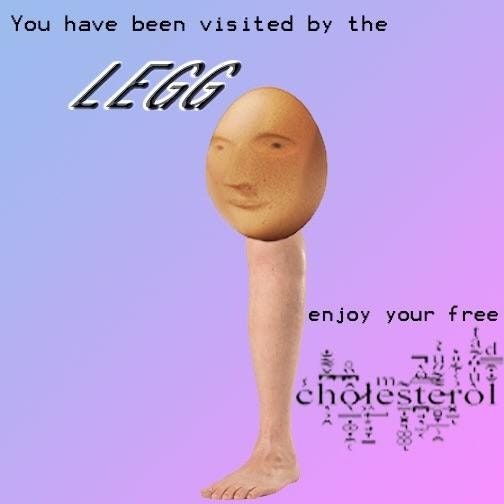
\includegraphics[width = 0.5\textwidth]{pictures/legg.jpg}
                    \caption{noga}
                    \label{fig:noga}
                \end{figure}
                \begin{figure}[htbp] 
                    \centering
                    
\includegraphics[width = \textwidth, scale = 2]{pictures/pain.jpg} %rozmiar obrazka w skali 2
                    \caption{pain}
                    \label{fig:pain}
                \end{figure}
\newpage
\subsection{Matematyka}
\begin{enumerate}
    \item Są macierze np: 
        $$\begin{bmatrix}
            a_(1, 1)&a_(1, 2)&...&a_(1, m)\\
            .&.&.&.\\
            .&.&.&.\\
            .&.&.&.\\
            a_(n, 1)&a_(n, 2)&...&a_(n,m)  
        \end{bmatrix}$$
    \item I układy równań mogą być też:
        $$\begin{cases}
            x^2 + 3y^7 + 9 +34x = 0\\
            x + y + 2 =8
        \end{cases}$$
    \item Całki i granice niestety też :(( \\
        \begin{math}
            \int 3x^2 \,dx = x^3 + C \\
            \lim_{x\to\infty} \frac{x^2 +3x -8}{6x^2 +7}
        \end{math}
    \item Wzory fizyczne też 
        \begin{equation}
            \oint_L \vec{E} \cdot \,d \vec{l} = - \frac{\, \Phi_B}{\, dt}
        \end{equation} 
        \[F_g = G \frac{mM}{R^3}\] %ponieważ nawiasy są kwadratowe wyrażenie znalazło się w następnej linijce, gdyby były okrągłe nie stałoby się to
\end{enumerate}

\subsection{Tabela}
Tabela \ref{tab:dlugopisy} przedstawia wyniki badań przeprowadzonych przez uczniów V liceum, w celu wybrania najoptymalniejszego długopisu do napisania matury w 2023 roku.
\begin{table}[htbp]
\centering

    \begin{tabular}{|c|c|c|c|c|c|}\hline
         \multicolumn{6}{|c|}{Ocena długopisów na maturę}\\\hline \hline 
                 Długopis&  Szybkość pisania&  Estetyka&  Rozmazywanie&  Czarność&  Pzryjemność\\ \hline 
                 Pilot 6-2 05&  7&  4&  2&  9&  5\\ \hline 
                 Milan P1 touch&  8&  8.5&  10&  7&  8.5\\ \hline
                 Pentel BK77& 8& 6& 10& 4&6\\\hline
                 Corwina 51C (1.0)& 9.5& 9& 10& 9&8.5\\\hline
                 InkJoy 100(paper mate)& 9& 9& 9& 9&9\\\hline
                 Pentel France& 9.5& 8& 10& 2.5&7\\\hline
    \end{tabular}
    \label{tab:dlugopisy}
    \caption{Ocena długopisów do napisania matury} 
\end{table}

\subsection{Dłuższy tekst}
\textbf{\textit{Historia o bucie, Shreku, oknie i pożarze}} \underline{(AI generated)}\\
\vskip
Pewnego dnia, Bucik, który był \emph{bardzo zadowolony ze swojego życia}, postanowił wyjść na spacer. Spacerował przez \textbf{las}, aż natknął się na \textbf{Shreka}. Shrek był \emph{bardzo zły}, ponieważ jego okno zostało zniszczone w \textbf{pożarze}. Bucik poczuł się bardzo źle i postanowił pomóc Shrekowi.\\
Bucik zaproponował, że \textit{może naprawić okno Shreka}. Shrek był bardzo zadowolony z tej propozycji i poprosił Bucika o pomoc. Bucik szybko naprawił okno i \underline{Shrek był bardzo wdzięczny}.

Shrek zaprosił Bucika do swojego domu na herbatę. Bucik był bardzo szczęśliwy, że mógł pomóc Shrekowi i spędzić czas z nim. Po herbacie Shrek powiedział Bucikowi, że jest bardzo wdzięczny za jego pomoc i że jest to dla niego bardzo ważne.
\underline{Bucik poczuł się bardzo dobrze} i wiedział, że \textit{zawsze} będzie mógł liczyć na \textbf{przyjaźń Shreka}.

\emph{I tak kończy się historia o bucie, Shreku, oknie i pożarze.}

\subsection{Lista}

\subsubsection{Top 3 najtrudniejsze przedmioty:}
\begin{enumerate}
    \item Analiza matematyczna
    \item Ćwiczenia z analizy matematycznej
    \item Analiza matematyczna 1
\end{enumerate}

\subsubsection{Lista życzeń dla św. Mikołaja:}
\begin{itemize}
    \item[--] Zrozumieć analize matematyczną
    \item[--] Zaliczyć ćwiczenia z analizy matematycznej
    \item[--] Zdać egzamin z analizy matematycznej
\end{itemize}
%\end{document}
